% vim: spelllang=es

\chapter{Entendiendo Tremor}\label{ch:tremor}

\section{Sistemas de Procesado de Eventos}

Tremor es un \emph{Sistema de Procesado de Eventos}, que consiste en ``el
monitorizado y análisis (procesado) de flujos de información (datos) sobre cosas
que pasan (eventos)''~\cite{luckham2011event}. Tremor fue creado como una
alternativa de alto rendimiento a herramientas como \textcite{logstash} o
\textcite{telegraf}, pero ha evolucionado para soportar casos de uso más
complejos. Al contrario que esas piezas de software, Tremor también tiene
soporte para \emph{agregación} y \emph{rollups}, e incluye un lenguaje \emph{ad
hoc} para \emph{Extract, Transform, and Load (ETL)} y consultas.

Para más información sobre Tremor se puede consultar \textcite{tremorintro}, que
contiene una explicación de sus conceptos más básicos y sus posibles usos --- o
cuándo \emph{no} usarlo, en \textcite{tremorconstraints}.
\textcite{tremorrecipes} lista un total de 32 ejemplos de cómo configurar y
emplear el software.

La figura~\ref{fig:tremor_example} ilustra uno de los casos de uso más básicos
de Tremor:

\begin{enumerate}
    \item Recibir \emph{logs} de varias aplicaciones en diferentes protocolos o
        formatos.
    \item Filtrar los casos redundantes, añadir campos y eliminar algunos
        innecesarios y transformar todo a un mismo formato.
    \item Enviar todos los logs estructurados a una base de datos para
        analizarlos posteriormente.
\end{enumerate}

\begin{figure}
    \centering
    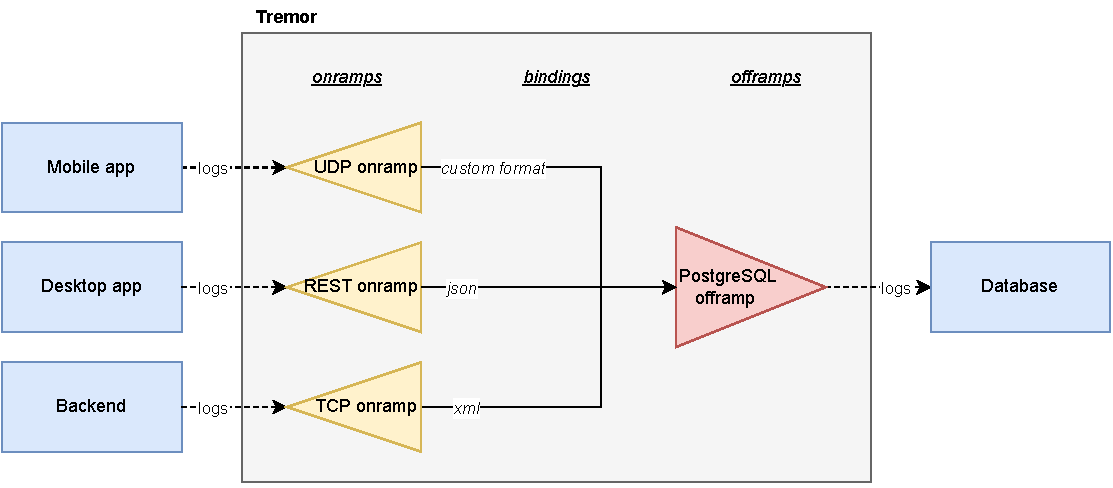
\includegraphics[width=\textwidth]{./Imagenes/example.pdf}
    \caption{Ejemplo de uso de Tremor}%
    \label{fig:tremor_example}
\end{figure}

Esto se basa en el concepto de \emph{onramps o sources} y \emph{offramps o
sinks}:

\begin{itemize}
    \item Una \onramp especifica cómo Tremor se conecta con el mundo exterior (o
        una \pipeline) para \textbf{recibir} de sistemas externos, como TCP,
        periódicamente, o PostgreSQL~\cite{tremoronramps}.

    \item Una \offramp especifica cómo Tremor se conecta con el mundo exterior
        (o una \pipeline) para \textbf{enviar} a sistemas externos, como
        \emph{stdout}, Kafka, o ElasticSearch~\cite{tremorofframps}.

    \item Una \pipeline es una lista de operaciones (transformación, agregación,
        eliminación, etc) a través de la cual se pueden encaminar los
        eventos~\cite{tremorpipelines}.

\end{itemize}

Sin embargo, es posible que algunas \onramps no solo quieran recibir de sistemas
externos, sino también responderles directamente, actuando como una \offramp, y
viceversa. En la versión 0.11 --- la presente cuando me uní al proyecto --- este
problema se solucionaba con el concepto de \emph{linked transports}. Estos son
especialmente útiles para \onramps y \offramps como REST y \websockets, donde el
protocolo da la posibilidad de responder a eventos usando la misma conexión, por
ejemplo con un ACK.

El término \connector se introdujo en mayo con la versión 0.12. Solucionan el
problema desde el inicio, abstrayendo tanto los \onramps como los \offramps bajo
el mismo concepto, incluyendo los \emph{linked transports}. Dado que estos
estaban siendo desarrollados mientras 0.11 era la última versión, el sistema de
plugins se enfocó a \connectors, en lugar de \onramps u \offramps, que ahora
están en desuso.

A nivel de implementación, los \connector se definen con el \trait
\code{Connector}, que se puede simplificar a:

\begin{minted}{rust}
pub trait Connector {
    /// Crea la parte "source" del conector, si es aplicable.
    async fn create_source(
        &mut self,
        _source_context: SourceContext,
        _builder: source::SourceManagerBuilder,
    ) -> Result<Option<source::SourceAddr>> {
        Ok(None)
    }

    /// Crea la parte "sink" del conector, si es aplicable.
    async fn create_sink(
        &mut self,
        _sink_context: SinkContext,
        _builder: sink::SinkManagerBuilder,
    ) -> Result<Option<sink::SinkAddr>> {
        Ok(None)
    }

    /// Intenta conectarse con el mundo exterior. Por ejemplo, inicia la
    /// conexión con una base de datos.
    async fn connect(
        &mut self,
        _ctx: &ConnectorContext,
        _attempt: &Attempt
    ) -> Result<bool> {
        Ok(true)
    }

    /// Llamado una vez cuando el connector inicia.
    async fn on_start(&mut self, _ctx: &ConnectorContext) -> Result<()> {
        Ok(())
    }
    /// Llamado cuando el connector pausa.
    async fn on_pause(&mut self, _ctx: &ConnectorContext) -> Result<()> {
        Ok(())
    }
    /// Llamado cuando el connector continúa.
    async fn on_resume(&mut self, _ctx: &ConnectorContext) -> Result<()> {
        Ok(())
    }
    /// Llamado ante un evento de "drain", que se asegura de que no
    /// lleguen más eventos a este conector.
    async fn on_drain(&mut self, _ctx: &ConnectorContext) -> Result<()> {
        Ok(())
    }
    /// Llamado cuando el conector para.
    async fn on_stop(&mut self, _ctx: &ConnectorContext) -> Result<()> {
        Ok(())
    }
    /// Devuelve los requerimientos para los códecs.
    fn codec_requirements(&self) -> CodecReq;
}
\end{minted}

\begin{figure}
    \centering
    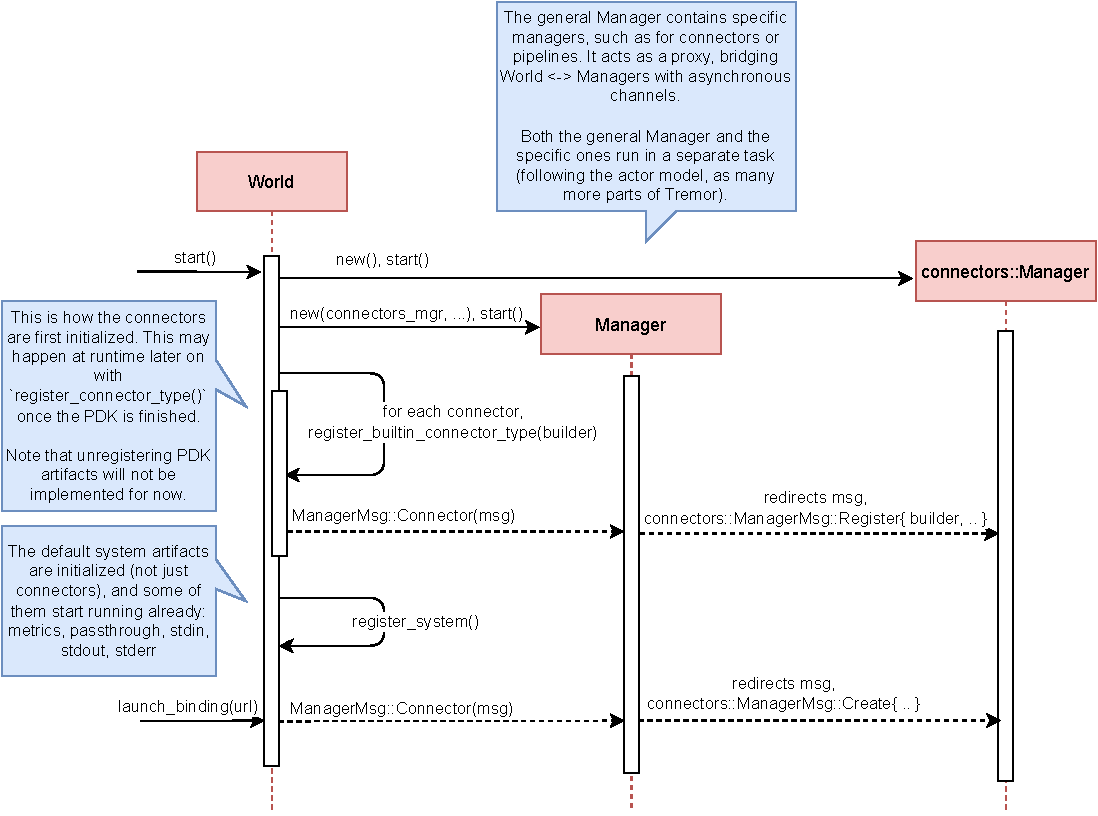
\includegraphics[width=\textwidth]{./Imagenes/registering.pdf}
    \caption{Ejemplo de uso de Tremor}%
    \label{fig:tremor_registering}
\end{figure}

\begin{figure}
    \centering
    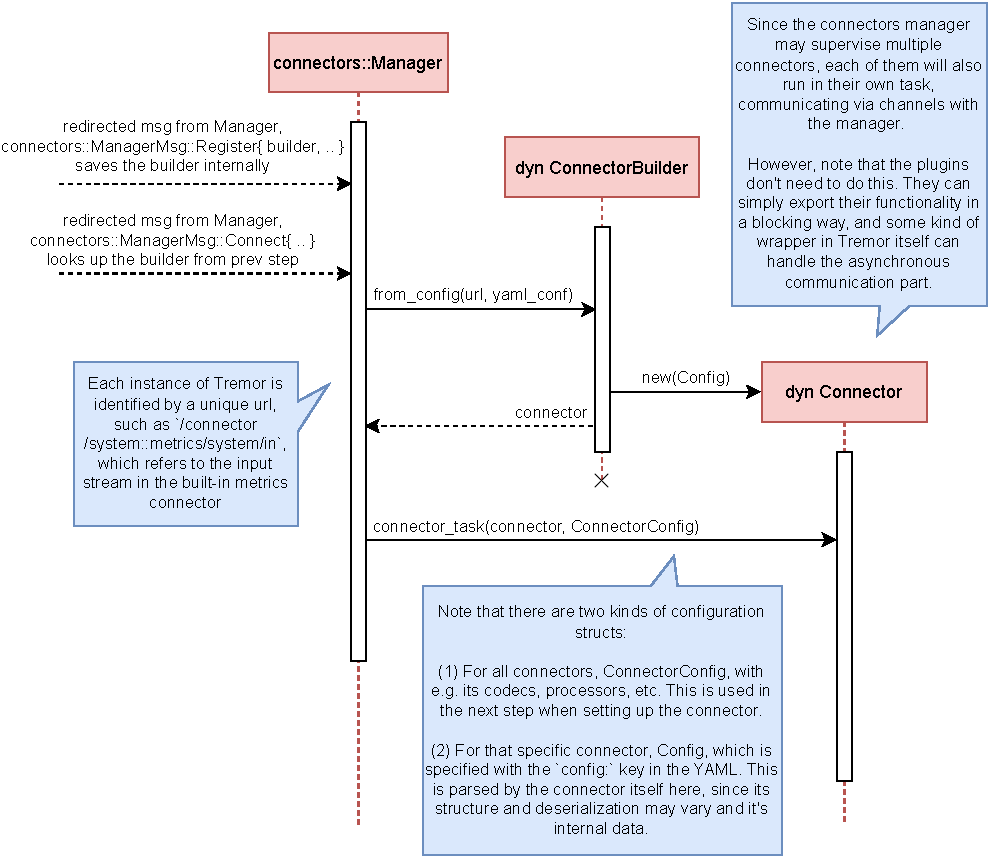
\includegraphics[width=\textwidth]{./Imagenes/initializing.pdf}
    \caption{Ejemplo de uso de Tremor}%
    \label{fig:tremor_initializing}
\end{figure}

\begin{figure}
    \centering
    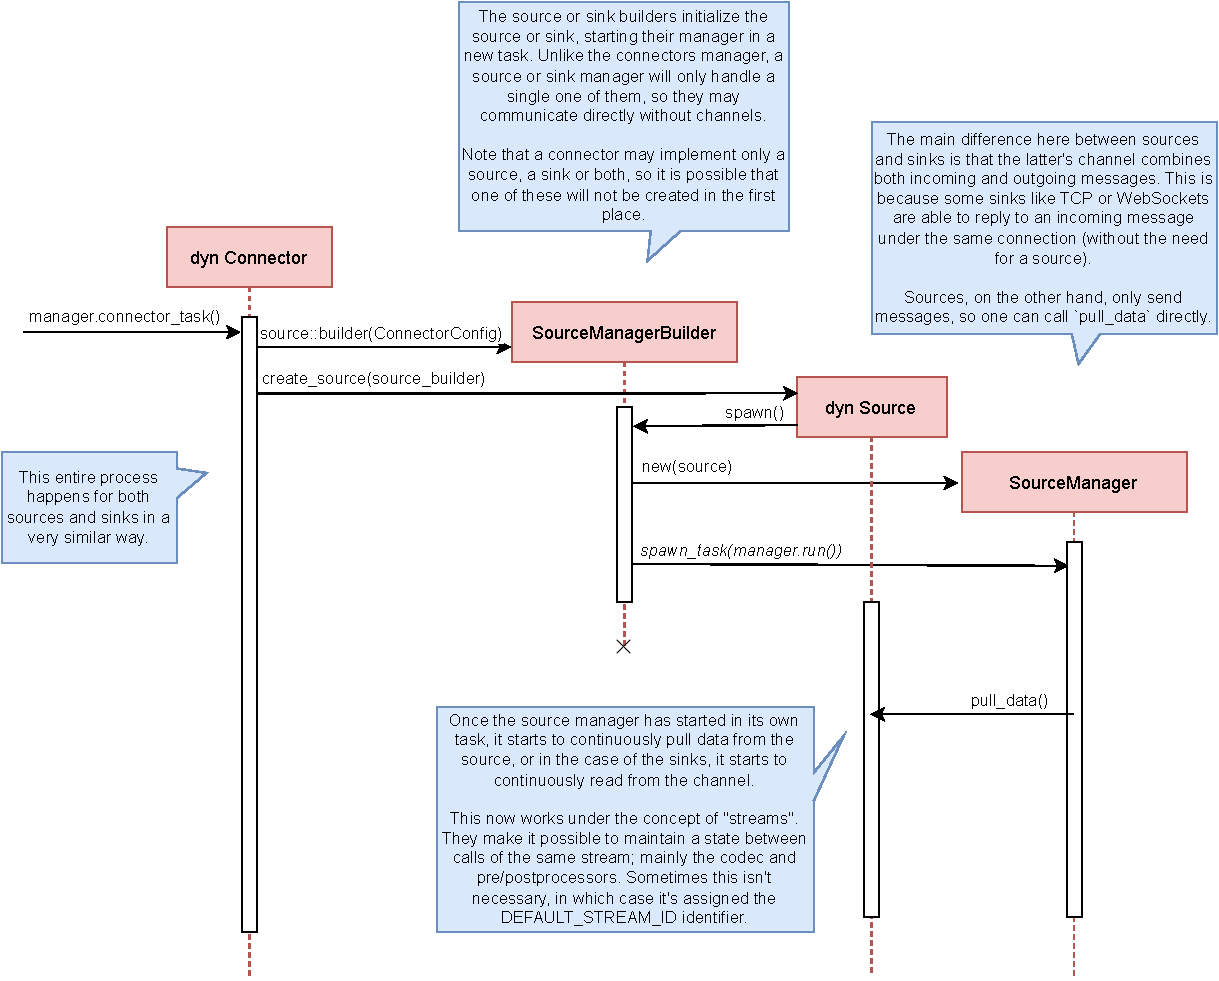
\includegraphics[width=\textwidth]{./Imagenes/setting-up.pdf}
    \caption{Ejemplo de uso de Tremor}%
    \label{fig:tremor_setting_up}
\end{figure}
